\chapter{Implementation and Validation}

I will not discuss the specific implementations in this thesis. For a detailed description of specific functions etc., see the the actual code for comments. The concept of this chapter is to give insight about the ideas behind the implementation.  Long story short, alot of hard work has been put into deep object orientation (for details, see Section~\ref{sec:OO}) in order to combine the different building blocks of QMC-methods in a natural and coherent way. As with all big coding projects, a major part of development went into planning and structuring.

\section{Structure and Implementation}
\label{sec:StructureandImplementation}

In QMC, Quantum Mechanics, and even physics in general, there are natural ways of decoupling the code in order to create a bridge between physics and code. Gathering data into objects representing physical concept to which a reader can relate increases the overall readability of the code. It also dramatically decreases the time it takes to implement or debug new methods, since mathematical intuition can be used in order to trace certain behaviours back to the source \footnote{For instance, if something is wrong with the sampling rule, a random walker might behave weird. The natural starting point of debugging is then the object in which the sampling rules are set. In the case of this thesis, this is the Sampling class containing a Diffusion object.}. Another reason is to generalize the code for several different cases, without having to rewrite or mess up anything (see the PotionGame example in Section~\ref{sec:PotionGame}).

\subsection{Methods used for Increasing Readability and Overall Structure}


As an example, the contents of the \verb+Walker+ class in Table ~\ref{tab:walkerClassMembers}. The idea behind this structure is that whenever we need a new walker in e.g. DMC, all we need to do is to create a new instance of \verb+Walker+. Deleting a walker is just as clean. A function which requires access to several elements from Table~\ref{tab:walkerClassMembers} now only requires one argument, namely the walker of interest. Let us look at an example


\vspace{0.5 cm}
\begin{lstlisting}
DMC::DMC(...) {

    ...
 
    original_walkers = new Walker*[spesify a number of walkers];
    
    ...

}
\end{lstlisting}


\begin{lstlisting}
void DMC::initialize() {

    ...

    //Initializing active walkers
    for (int k = 0; k < n_w; k++){
        original_walkers[k] = new Walker(n_p, dim);
    }
    
    //Seting trial position of active walkers
    ...

    //Calculating and storing energies of active walkers
    for (int k = 0; k < n_w; k++) {
        calculate_energy_necessities(original_walkers[k]);
        original_walkers[k]->set_E(calculate_local_energy(original_walkers[k]));
    }

    ...

}
\end{lstlisting}

\begin{table}

 \begin{center}

 \begin{tabular}{|c l l|}
 \hline
 Type & Name & Description \\
 
 \hline
 \hline
 
 \verb+mat+         & \verb+r+             & The position.\\

 \hline
 \hline
 
 \verb+mat+         & \verb+r_rel+         & The relative positions.\\
 \verb+rowvec+      & \verb+ r2+           & The squared positions. \\
 \verb+mat+         & \verb+phi+           & The last evaluated single particle orbitals. \\
 \verb+field<mat>+  & \verb+dell_phi+      & The last evaluated gradients of the single particle orbitals. \\
 \verb+cube+        & \verb+dJ+            & The last evaluated terms of the jastrow factor derivatives. \\
 \verb+mat+         & \verb+spatial_grad+  & The gradient of the uncorrelated wave function.\\
 \verb+mat+         & \verb+jast_grad+     & The gradient of the Jastrow factor.\\
 \verb+mat+         & \verb+inv+           & The inverse of the slater matrix.\\
 \verb+mat+         & \verb+qforce+        & The quantum force.\\
 
 \hline 
 \hline
 
 \verb+double+      & \verb+spatial_ratio+ & The current ratio between this walker and another walker.\\
 \verb+double+      & \verb+value+         & The value of the wave function.\\
 \verb+double+      & \verb+lapl_sum+      & The full Laplacian of the wave function.\\
 \verb+double+      & \verb+E+             & The energy of the walker. \\
 \verb+bool+        & \verb+is_murdered+   & A flag for the DMC brancing algorithm. \\
 \hline 
 \end{tabular}
 
 \caption{Description of the members of the Walker class. All matrices holds information on all particles.
The second block corresponds to vectors kept in memory to avoid expensive recalulation. The third block corresponds to  scalar values calculated and kept in memory for later use or control.}
 \label{tab:walkerClassMembers}
 
 \end{center}
\end{table}

Initializing new walkers is, as seen above, unproblematic. Calculating values in the machinery now always involves a corresponding walker. For instance, when looping over walkers in DMC, the amount of juggling is reduced to nothing; all you need to do is to loop over a vector of walkers. This walker can then be sent to any function, resulting in code like e.g.

\vspace{0.5cm}
\begin{lstlisting}
double Coulomb::get_pot_E(const Walker* walker) const {
    
    double e_coulomb = 0;

    for (int i = 0; i < n_p - 1; i++) {
        for (int j = i + 1; j < n_p; j++) {
            e_coulomb += 1 / walker->r_rel(i, j);
        }
    }

    return e_coulomb;
}
\end{lstlisting}

The alternative to the code above is to juggle one relative position matrix per walker, ruining both the readability and the overall structure of the code. Another upside to this way of structuring, is that we can tie the source code and the method description closer together. Look at VMC as an example. VMC uses a walker and a trial walker. 

\vspace{0.5cm}
\begin{lstlisting}
void VMC::initialize() {
    
    ...

    sampling->set_trial_pos(original_walker);
    copy_walker(original_walker, trial_walker);
    
    ...
    
}

\end{lstlisting}

Another example where object orientation dramatically increases the readability of the code is the interplay between the Sampling- and Diffusion-class. From \textbf{REF TO THEORY} we know that if we use importance sampling, the diffusion follows the Fokker-Planck equation (Eq.~\textbf{CITE EQ FOKKERPLANCK}). The implementation is as follows:

\vspace{0.5cm}
\begin{lstlisting}
Importance::Importance(GeneralParams & gP)
: Sampling(gP.n_p, gP.dim) {

    diffusion = new Fokker_Planck(n_p, dim, gP.random_seed);

}
\end{lstlisting}


\subsection{Methods for Generalizing the Code}

The importance sampling constructor serves as a good example in this case as well. A \verb+Sampling+ object type might be an instance of \verb+Importance+ or \verb+Brute_Force+, however, we do not need to know this in order to abstractly describe how to diffuse a walker. We do not even need to know whether we are doing VMC or DMC. All we need to know is that the \verb+Diffusion+ object within the sampling holds the rules we need once the correct objects are in place. This is reflected in the following code:

\vspace{0.5cm}
\begin{lstlisting}
void Sampling::update_pos(const Walker* walker_pre, Walker* walker_post, int particle) const {

    for (int j = 0; j < dim; j++) {
        walker_post->r(particle, j) = walker_pre->r(particle, j)
                + diffusion->get_new_pos(walker_pre, particle, j);
    }

    //more updates through jastrow pointers etc.
    ...

}
\end{lstlisting}

\begin{lstlisting}
double Diffusion::get_new_pos(const Walker* walker, int i, int j) {
    return gaussian_deviate(&random_seed) * std;
}

double Simple::get_new_pos(const Walker* walker, int i, int j) {
    return Diffusion::get_new_pos(walker, i, j);
}

double Fokker_Planck::get_new_pos(const Walker* walker, int i, int j) {
    return D * timestep * walker->qforce(i, j) + Diffusion::get_new_pos(walker, i, j);
}
\end{lstlisting}

This use of polymorphism (as described in Section \ref{sec:typeCastPoly}) is widely used throughout the code to generalize it. As a goal, the idea was to produce a code with the following generalizations:

\begin{itemize}
 \item As many as possible functions should be written generally for DMC and VMC.
 \item Objects should not assume the type of any sub-classed object except its own, unless the type is directly implied (importance sampling implies Fokker-Planck diffusion), i.e., deep polymorphism.
\end{itemize}

This puts a series of constraints on the code; it should be general for (in any combination):

\begin{enumerate}[label=(\roman{*}), ref=(\roman{*})]
\item No trailing if-tests or flags handling switched cases. A single test in the main file decides everything once and for all. 
\item Importance- and Brute Force-sampling.
\item Numerical or closed form expressions for the kinetic energy and quantum force.
\item Fermions and Bosons.
\item Any choice of single particle basis, included expanded bases.
\item Functionality to add any combination of any potential.

\end{enumerate}


\subsubsection{Constraints (i) - (iv)}

As mentioned previously, \verb+QMC+ holds an object of type \verb+Sampling+, which contains all the general functions for diffusing particles and how to sample them. It also ensures that the walker holds the necessary data in order to continue the sampling, e.g. the Quantum Force if we do importance sampling. This is achieved by having a pure virtual function \verb+get_necessities+, which is overrided by the subclasses \verb+Importance+ and \verb+Brute_Force+. In other words: The class structure is set up in such a way that the distinct parts which needs to be general are separated. Polymorphism takes care of the distinction, hence no if-tests are required. Below follows a part of the code illustrating this; the code for copying walkers, calculating energy necessities etc. follows the same idea.

\vspace{0.5cm}
\begin{lstlisting}
void Sampling::update_pos(const Walker* walker_pre, Walker* walker_post, int particle) const {

    //Positions and orbitals are updated for the particle at hand
    ...

    //updates the inverse slater in case of a fermion system
    qmc->get_system_ptr()->calc_for_newpos(walker_pre, walker_post, particle);

    //pure virtual function. Function will update quantum force if importance sampling.
    update_necessities(walker_pre, walker_post, particle);

}
\end{lstlisting}

In the case of numerical energy calculations, the function which evaluates the gradients can be set to a general numerical function (assuming the standard single particle orbitals are implemented). If the closed form expressions are implemented, these can be accessed directly instead. Fermions and bosons have different implementations of e.g. the spatial ratio of a wavefunction.


\subsubsection{Constraint (v)}

A single particle orbital is nothing but a function of a walker's coordinates and variational parameters.  An if-test hierarchy on the Quantum Number is the simplest way to implement a single particle basis, however, they can all be avoided using polymorphism. The class \verb+BasisFunctions+ represents an abstract function, which can takes on input a walker and evaluates an arbitrary expression. A subclass will hold the specific implementation, e.g. the first excited level of a harmonic oscillator.

\vspace{0.5cm}
\begin{lstlisting}
class BasisFunctions {
public:
    BasisFunctions();
    
    virtual double eval(const Walker* walker, int i) = 0;
};

double alphaHO_3::eval(const Walker* walker, int i) {
    
    //4*k2*y2 - 2
    H = 4*(*k2)*walker->r(i, 1)*walker->r(i, 1) - 2;
    return H * (*exp_factor);
    
}
\end{lstlisting}

These functions are loaded into an array representing the single particle basis in the \verb+Orbitals+ class' constructor.

\vspace{0.5cm}
\begin{lstlisting}
AlphaHarmonicOscillator::AlphaHarmonicOscillator(GeneralParams & gP, VariationalParams & vP)
: Orbitals(gP.n_p, gP.dim) {

    //Creating pointers in order to link the Orbital and BasisFunction parameters.
    this->alpha = new double();
    this->k = new double();
    this->k2 = new double();
    this->exp_factor = new double();

    this->w = gP.systemConstant;
    set_parameter(vP.alpha, 0);
    get_qnums();

    basis_functions[0] = new alphaHO_0(k, k2, exp_factor);
    basis_functions[1] = new alphaHO_1(k, k2, exp_factor);
    basis_functions[2] = new alphaHO_2(k, k2, exp_factor);
    basis_functions[3] = new alphaHO_3(k, k2, exp_factor);
    ...
    
\end{lstlisting}

All orbital files are generated automatically by a Python-script. The reasoning behind the unset pointers are to create a link between the parameters in \verb+BasisFunctions+ and \verb+Orbitals+, such that we do not have to change the value in all of the basis function objects (60 for 30 particles), we simply have to change the value in the orbitals class and the rest will follow.

With this rigid setup, evaluating orbitals can now we done in the following manner (similar for the gradient and Laplace)

\vspace{0.5cm}
\begin{lstlisting}
virtual double phi(const Walker* walker, int particle, int q_num) {
    return basis_functions[q_num]->eval(walker, particle);
}
\end{lstlisting}

The reason why \verb+phi+ is a virtual function, is so that the \verb+ExpandedBasis+ class can override it. With this systematic setup of single particle orbitals, it is very simple and intuitive to implement the expanded basis functionality

\vspace{0.5cm}
\begin{lstlisting}[language=C++]
class ExpandedBasis : public Orbitals {

...

protected:

    int basis_size;
    arma::mat coeffs;
    Orbitals* basis;

};

ExpandedBasis::ExpandedBasis(GeneralParams & gp, Orbitals* basis, int basis_size, std::string coeffPath)
: Orbitals(gp.n_p, gp.dim) {

    this->basis = basis;
    this->basis_size = basis_size;
    coeffs = arma::zeros<arma::mat > (n2, basis_size);

    //read coefficients

}

\end{lstlisting}

The expanded basis class is implemented as a subclass to the original orbital class, however, it is designed to work along side it. Instead of a list of orbital basis functions, it holds a \verb+Orbital+ object, containing the basis in which we want to expand, alongside a matrix containing the coefficients of expansion. Implementing the new single particle functions is simply done by virtual function overriding as below: 

\vspace{0.5cm}
\begin{lstlisting}

double ExpandedBasis::phi(const Walker* walker, int particle, int q_num) {

    double value = 0;
    for (int m = 0; m < basis_size; m++) {
        value += coeffs(particle, m) * basis->phi(walker, particle, m);
    }

    return value;

}
\end{lstlisting}

And of course similarly for the gradient and Laplace. The expression is very close to the raw mathematical description of a basis expansion. 

\subsubsection{Constraint (vi)}

When we are loading a set of single particle states, we are loading those who best match the given Hamiltonian of our system. For quantum dots, we load harmonic oscillator states, for atoms we load hydrogen states and so on. By having great flexibility in both the Hamiltonian and the basis functions means the code is easily adaptable to other systems. The flexibility of the potential class is already discussed in Section \ref{sec:typeCastPoly}.

The complete list of classes working in the same way (iteration over loaded elements, no if-tests) is


\begin{listliketab}
\storestyleof{itemize}
 \begin{tabular}{l l}
  \textbullet \,\verb+Potential+         & See section \ref{sec:typeCastPoly} for detials. \\
  \textbullet \,\verb+ErrorEstimator+:   & Initialized to \verb+Blocking+ or \verb+SimpleVar+. Samples data.\\
  \textbullet \,\verb+OutputHandler+:    & Saves specified data to a specified file, e.g. \verb+stdoutDMC+.\\
 \end{tabular}
\end{listliketab}


Creating optimized and general code takes longer to develop, but pays off when it comes to later implementations of extensions to the library.

\subsection{Visualization}
DCVIZ?

\section{Performance Optimizations}

\subsection{RAM use}

the RAM use of VMC is close to nothing; we only have two walkers with each their set of matrices. However, DMC has the potential to use a lot of RAM, as thousands of walkers are allocated. The walkers account for close to all of the RAM used by the methods, as the rest of the framework consist only of a small amount of doubles (8 bytes) and integers (4 bytes). A short analysis of the RAM spent per \verb+Walker+ object yields

\begin{listliketab}
\storestyleof{itemize}
 \begin{tabular}{l l}
  \textbullet 1 boolean                                        & 1 byte                                \\
  \textbullet 3 integers                                       & 12 bytes                              \\
  \textbullet 3 doubles                                        & 24 bytes                              \\
  \textbullet 4 \verb+n_p+ $\times$ \verb+dim+ matrices        & 32 \verb+n_p+ $\cdot$ \verb+dim+ bytes\\
  \textbullet 1 \verb+n_p+ $\times$ \verb+n_p+ matrix          & 8 \verb+n_p+ $\cdot$ \verb+n_p+ bytes \\
  \textbullet 2 \verb+n_p+ $\times$ \verb+n_p/2+ matrices        & 4 \verb+n_p+ $\cdot$ \verb+n_p+ bytes \\
  \textbullet 1 array of length \verb+n_p+                     & 8 \verb+n_p+ bytes                    \\
  \textbullet 1 field of length \verb+n_p+                     & 8 \verb+n_p+ bytes                    \\
  \textbullet 1 \verb+n_p+ $\times$ \verb+n_p/2+ $\times$ \verb+dim+ field & 8 \verb+n_p+ bytes                    \\
  \textbullet 1 \verb+n_p+ $\times$ \verb+n_p+ $\times$ \verb+dim+ cube & 8 \verb+n_p+ bytes\\
  Total:                                                       & 37 + 32 \verb+n_p+ $\cdot$ \verb+dim+ + 12 \verb+n_p+ $\cdot$ \verb+n_p+ + 8 \verb+n_p+ bytes \\
 \end{tabular}
\end{listliketab}

For VMC with 30 particles and quantum dots in 2 dimensions this gives a walker RAM usage of 25 kB, which is practically nothing. For DMC however, we have e.g. 1000 active walkers and 4000 inactive. The inactive ones can be left uninitialized, saving the RAM of all matrix initializations (37 RAM per walker). 

In Figure~\ref{FIG:RAMusageDMC} we see how the RAM usage in a typical DMC calculation scales with the number of particles. For 30 particles, we have approximately 60 MB of RAM spent on walkers. This is still practically nothing compared to the available RAM on modern computers (minimum 2 GB).

\begin{figure}
\label{FIG:RAMusageDMC}
 \begin{center}
  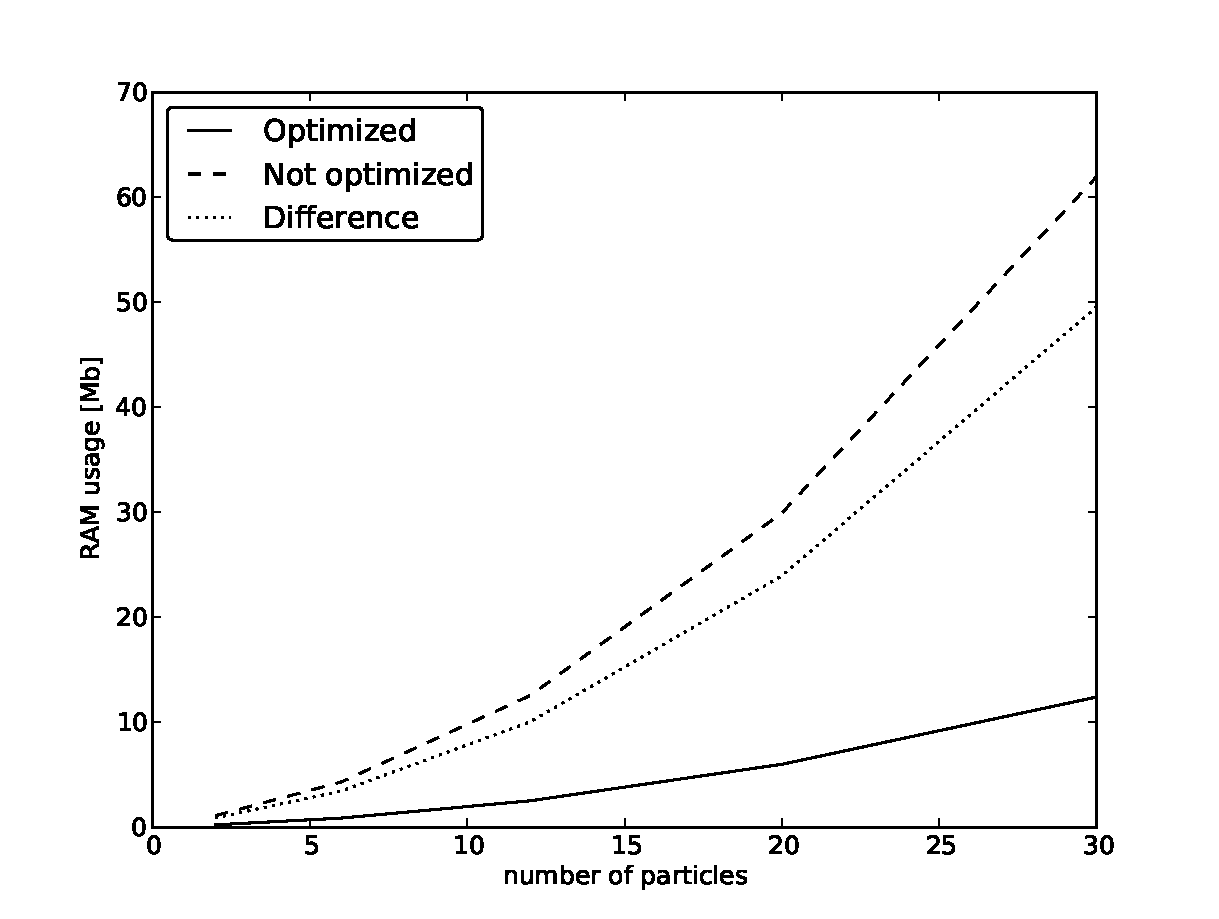
\includegraphics[scale=0.75]{../Graphics/RAMusagePrWalker.pdf}
  \caption{Number of particles vs. the theoretical RAM usage in a typical DMC run for the optimized and unoptimized case. Calculated for two dimensions, 1000 active walkers and 5000 inactive.}
 \end{center}
\end{figure}

The conclusion stands that as long as there are no memory leaks, time spent optimizing the memory use is time wasted. Memory optimizations might damage the readability, so the code was left more or less unoptimized in this part.

\subsection{CPU-time}
Looking at Table \ref{tab:walkerClassMembers}, the only thing we have to store in order for the machinery to work is the position matrix. Every other matrix is initialized to optimize CPU time.

During a Quantum Monte Carlo sampling process, certain values, such as the relative distances, are used to calculate quantities such as the energy. The most brute force way of handling situations like this is to calculate everything at the time it is needed. However, once a diffusion step is made,we use the same relative distances both in the Jastrow factor and its gradient. Calculating them twice is a waste of time. We can instead store them in a matrix, and access this matrix in both functions:

\[
r_{rel} = r_{rel}^T = \left( \begin{array}{ccccc}
0 & r_{12} & r_{13} & \cdots & r_{1N} \\
 & 0 & r_{23} & \cdots & r_{2N}  \\
 &  & \ddots & \ddots & \vdots \\
 & \cdots &  & 0 & r_{(N-1)N} \\
 &  &  &  & 0\end{array} \right).
\]

Another upside with this way of storing the relative distances, is that moving particle $i$ in our code, only changes the $i$'th row in the matrix, and therefore we need only to recalculate \textit{N} elements (\textit{N} being the number of particles in our system). For the same reason, storing the gradients, Laplacian sums and the squared radii is matrices also optimize the code. 

Having closed form expressions for the gradients and Laplacians for the different parts of the wave function is another source of dramatic speed-up. The local kinetic energy ($(E_k)_L$) and the Quantum Force ($\mathbf{F}_i$) can be expressed in terms of the separate parts of the wave function:

\begin{eqnarray}
(E_k)_L &=& -\frac{1}{2}\frac{1}{\psi_T}\nabla_i^2 \psi_T \\
&=& -\frac{1}{2}\frac{1}{|S|\psi_C}\nabla_i^2(|S|\psi_C) \nonumber\\
&=& -\frac{1}{2}\frac{1}{|S|\psi_C} \nabla_i \left(\psi_C\nabla_i |S| + |S|\nabla_i \psi_C\right)\nonumber  \\
&=& -\frac{1}{2}\Big[\frac{1}{\psi_C}\nabla_i^2 \psi_C + \frac{2}{|S|\psi_C}\nabla_i|S|\cdot\nabla_i\psi_C \nonumber\\
&& \qquad\qquad\qquad\,\,+\frac{1}{|S|}\nabla_i^2 |S|\Big].\nonumber 
\label{eq:kinetic_analytic}
\end{eqnarray}

\begin{eqnarray}
 \mathbf{F}_i &=& \frac{2}{|S|\psi_C}\nabla_i( |S|\psi_C) \\
&=& 2\left(\frac{1}{\psi_C}\nabla_i \psi_C + \frac{1}{|S|}\nabla_i |S|\right),\nonumber
\label{eq:QF}
\end{eqnarray}
where $i$ denotes particle number, and $|S|$ and $\psi_C$ are respectively the spatial wave function and the Jastrow factor.

For Fermions, it can be shown that we have the following relations for the Slater determinant\cite{larseivind}:

\begin{eqnarray}
 \frac{1}{|S|}\nabla_i |S| &=& \displaystyle\sum_{j=1}^n \nabla_i \phi_j(\vec r_i)S^{-1}_{ji} \\ 
\frac{1}{|S|}\nabla^2_i |S| &=& \displaystyle\sum_{j=1}^n \nabla^2_i \phi_j(\vec r_i)S^{-1}_{ji},\nonumber
\label{eq:grad_lapl_S}
\end{eqnarray}
where $S^{-1}$ is the inverse of the Slater matrix, and $n$ is the dimensionality of the Slater matrix, in our case $n=N/2$, where $N$ is the number of electrons. $\phi_j(\vec r_i)$ are the single-particle basis functions, where $j$ denotes the quantum numbers. For example $j=0$ is the ground state, $j=1$ first excited state and so on. 

These values of the gradient and Laplacian of the single-particle wave functions needs to be tabulated. Most of the single particle bases used are expressed using simple mathematics, such as Hermite polynomials for the case of harmonic oscillator, and the derivatives can therefore be calculated pretty easily. 

Calculating an inverse does not seem to optimize much. However, we can run an updating algorithm for the inverse, which ends up saving a lot of time. The ratio of the spatial determinants can also be expressed using this inverse\cite{larseivind}. This means that no explicit wave function calculation is needed (we can calculate the ratio between two Jastrow factors without problem). The expression for the ratio in terms of the inverse is
\begin{equation}
 R_S = \displaystyle\sum_{j=1}^n \phi_j({\vec r}_{i,\mathrm{new}})S^{-1}_{ji}(\vec r_\mathrm{old}),
\label{eq:Ratio}
\end{equation}
where $i$ is the particle being moved.

In the case of $s=\frac{1}{2}$-Fermions, the code holds two slater determinants (spin up and down); we need two inverse matrices. All if-tests on whether or not to access spin up or down is however avoided by merging the two inverse matrices into one augmented matrix

\[
 S^{-1} = \left[S^{-1}_\uparrow S^{-1}_\downarrow\right].
\]

\noindent
This way of storing the data completely removes the need of if-tests on spin.

Updating the inverse matrix can be done once we got the new position and the ratio

\begin{eqnarray}
 S^{-1}_{kj}(\vec r_\mathrm{new})  = \left\{ 
\begin{array}{l l}
  S^{-1}_{kj}(\vec r_\mathrm{old}) - \frac{1}{R_S}S^{-1}_{ki}(\vec r_\mathrm{old})\displaystyle\sum_{l=1}^{n} \phi_{l}(\vec r_{i,\,\mathrm{new}})  S^{-1}_{lj}(\vec r_\mathrm{old}) &\qquad \mbox{$j \neq i$} \\
 \frac{1}{R_S}S^{-1}_{ki}(\vec r_\mathrm{old})  &\qquad \mbox{$j=i$}
\end{array} \right.
\label{eq:Update_inv}
\end{eqnarray}


Equal expressions like the the ones listed in Eq.~(\ref{eq:grad_lapl_S}) can be found for the case of the Pade-Jastrow factor as well:

\begin{eqnarray}
 \frac{1}{\psi_C^{PJ}}\nabla_i \psi_C^{PJ} &=& \displaystyle\sum_{j\ne i} \frac{\vec r_{ij}}{r_{ij}}\frac{a_{ij}}{(1+\beta r_{ij})^2} \\
\label{eq:grad_jast}
 \frac{1}{\psi_C^{PJ}}\nabla_i^2 \psi_C^{PJ} &=& \left|\frac{1}{\psi_C^{PJ}}\nabla_i \psi_C^{PJ}\right|^2 + 2\displaystyle\sum_{i < j} \frac{a_{ij}(1 - \beta r_{ij})}{r_{ij}(1 + \beta r_{ij})^3}. \nonumber
\label{eq:lapl_jastrow}
\end{eqnarray}

Notice that $a_{ij}$ is written as a matrix element. If we were to calculate $a$ for every single run in the loop, the double if-tests would drain a lot of CPU time. Prior to the sampling, in the \verb+Jastrow::initialize+ function, the values of $a$ are generated once and for all and stored in a matrix. This matrix remains unchanged throughout the entire sampling, and no if-tests are necessary.

For the simplest case of single particle harmonic oscillator basis functions (Eq.~(\textbf{REF OSC BASIS}), the expressions for the derivatives of the wave function with respect to the variational parameters is
\begin{eqnarray}
\frac{1}{\psi_T}\frac{\partial\psi_T}{\partial\alpha} &=& -\frac{1}{2}\omega\displaystyle\sum_{i=1}^N r_i^2, \\
\frac{1}{\psi_T}\frac{\partial\psi_T}{\partial\beta} &=& -\displaystyle\sum_{i<j}\frac{a_{ij}r_{ij}^2}{(1+\beta r_{ij})^2}.
\label{eq:CGM_derivatives}
\end{eqnarray}

which can be used to speed up the process of minimizing.


Optimization (without approximations) is all about not calculating more than you have to. Calculating gradients is the part of the code which require the most CPU time. The most time consuming functions is the gradients. Looking at Eq.~(\ref{eq:grad_lapl_S}) this comes as no surprise; the single particle wave functions contain a call to the exponential function, which is terribly slow and needs to be deadly accurate. The time consumption in the Jastrow gradient arise from the fact that once a particle is moved, the entire gradient changes. 

\section{Validation}

things should not be wrong. It is bad.


test:
\newpage
\begin{table}
\begin{center}
\label{tab:DMCRes}
\begin{tabular}{cc|cccc}
    N     & $\omega$ & $\mathrm{E_{VMC}}$ & $\mathrm{E_{DMC}}$ & $\alpha$ & $\beta$  \\
\hline
    2     &   0.28   & 1.02197  &  1.0216  & 0.970202 & 0.254158 \\
          &   0.5    & 1.66023  & 1.65994  & 0.981901 & 0.312174 \\
          &   1.0    & 3.00054  & 3.00002  & 0.988761 & 0.398956 \\
    6     &   0.28   & 7.62259  & 7.59967  & 0.87322  & 0.322838 \\
          &   0.5    & 11.8092  & 11.7845  & 0.896501 & 0.411444 \\
          &   1.0    & 20.1896  & 20.1606  & 0.920368 & 0.55734  \\
    12    &   0.28   & 25.7088  & 25.63814 & 0.797355 & 0.365122 \\
          &   0.5    & 39.2395  & 39.15974 & 0.859145 & 0.481956 \\
          &   1.0    & 65.7958  & 65.70032 & 0.873605 & 0.656703 \\
\end{tabular}
\caption{J. Hogberget}
\end{center}
\end{table}

\begin{table}
\begin{center}
\label{tab:LohneRes}
\begin{tabular}{cc|cccc}
    N     & $\omega$ & $\mathrm{E_{DMC}}$  \\
\hline
    2     &   0.28   &  N/A     \\
          &   0.5    & 1.65975(2)  \\
          &   1.0    &  3.00000(3) \\
    6     &   0.28   &   7.6001(1) \\
          &   0.5    &  11.7888(2) \\
          &   1.0    &  20.1597(2) \\
    12    &   0.28   &  25.6356(1) \\
          &   0.5    &  39.159(1)  \\
          &   1.0    &  65.700(1)  \\
\end{tabular}
\caption{M. Pedersen Lohne et al.}
\end{center}
\end{table}

\begin{table}
\begin{center}
\label{tab:noColValid}
\begin{tabular}{cc|ccc}
    N     & $\omega$ & $\mathrm{E_{VMC}}$ & $\mathrm{E_{DMC}}$ & $\alpha$ \\
\hline
    2     &   0.5    &   1.0    &   1.0    &   1.0    \\
          &   1.0    &   2.0    &   2.0    &   1.0    \\
    6     &   0.5    &   5.0    &   5.0    &   1.0    \\
          &   1.0    &   10.0   &   10.0   &   1.0    \\
    12    &   0.5    &   14.0   &   14.0   &   1.0    \\
          &   1.0    &   28.0   &   28.0   &   1.0    \\
    20    &   0.5    &   30.0   &   30.0   &   1.0    \\
          &   1.0    &   60.0   &   60.0   &   1.0    \\
    30    &   0.5    &   55.0   &   55.0   &   1.0    \\
          &   1.0    &  110.0   &  110.0   &   1.0    \\
\end{tabular}
\caption{}
\end{center}
\end{table}


